\documentclass[12pt,a4paper]{article}
\usepackage[top=16mm,bottom=18mm,left=16mm,right=16mm,headheight=0pt,headsep=0mm,footskip=10mm]{geometry}
\usepackage{iftex}
\ifPDFTeX
  \usepackage[utf8]{inputenc}
  \usepackage[T5]{fontenc}
  \usepackage{mathptmx}
\else
  \usepackage{fontspec}
  \usepackage{mathptmx}
  \IfFontExistsTF{Times New Roman}{\setmainfont{Times New Roman}}{\IfFontExistsTF{Tinos}{\setmainfont{Tinos}}{\setmainfont{TeX Gyre Termes}}}
\fi
\usepackage{amsmath,amssymb}
\usepackage{xcolor,tikz,graphicx,array,tabularx,enumitem,fancyhdr,lastpage}

% Phong cach theo BTVN_Luong_giac_B5.tex (de so 05 trong repository).
% Noi dung: De tu luyen TDM11X31 - Co ban ve hinh hoc khong gian.
% Hinh minh hoa cau 4 va 5 duoc ve lai bang TikZ, khong can tep anh ngoai.
\definecolor{questionpurple}{RGB}{137,38,143}
\definecolor{answerblue}{RGB}{35,45,140}
\setlength{\parindent}{0pt}
\setlength{\parskip}{0pt}
\renewcommand{\baselinestretch}{1.08}
\pagestyle{fancy}
\fancyhf{}
\renewcommand{\headrulewidth}{0pt}
\fancyfoot[L]{\small Toán 11 -- Hình học không gian}
\fancyfoot[R]{\small Trang \thepage/\pageref{LastPage} -- Đề test số 07}
\renewcommand{\footrulewidth}{.4pt}

\newlist{questions}{enumerate}{1}
\setlist[questions]{label=\textcolor{questionpurple}{\bfseries Câu \arabic*.},
 leftmargin=0pt,itemindent=16mm,labelwidth=14mm,labelsep=2mm,align=left,
 itemsep=4pt,topsep=3pt,parsep=0pt}
\newcommand{\answerlabel}[1]{\tikz[baseline=(choice.base)]\node[
 draw=black!65,text=answerblue,circle,inner sep=0pt,minimum size=4.8mm,
 line width=.4pt,font=\normalsize] (choice) {#1};}
\newcommand{\fourchoices}[4]{\par\begingroup\small
 \setlength{\tabcolsep}{0pt}\renewcommand{\arraystretch}{1.32}
 \begin{tabularx}{\linewidth}{@{}*{4}{>{\raggedright\arraybackslash}X}@{}}
 \answerlabel{A}~#1 & \answerlabel{B}~#2 &
 \answerlabel{C}~#3 & \answerlabel{D}~#4
 \end{tabularx}\endgroup}
\newcommand{\twochoices}[4]{\par\begingroup\small
 \setlength{\tabcolsep}{2pt}\renewcommand{\arraystretch}{1.37}
 \begin{tabularx}{\linewidth}{@{}*{2}{>{\raggedright\arraybackslash}X}@{}}
 \answerlabel{A}~#1 & \answerlabel{B}~#2\\
 \answerlabel{C}~#3 & \answerlabel{D}~#4
 \end{tabularx}\endgroup}
\newcommand{\tdm}[1]{{\small\textcolor{answerblue}{[#1]}}}

\begin{document}
\noindent
\begin{minipage}[t]{.35\textwidth}
  \centering
  {\bfseries CHUYÊN ĐỀ -- TOÁN -- 11\par}
  \vspace{2pt}\rule{.72\linewidth}{.4pt}\par\vspace{3pt}
  HÌNH HỌC KHÔNG GIAN\par\vspace{4pt}
  {\itshape ĐỀ TEST SỐ 07\par}
\end{minipage}\hfill
\begin{minipage}[t]{.62\textwidth}
  \centering
  {\bfseries CƠ BẢN VỀ HÌNH HỌC\par
  KHÔNG GIAN\par}
  \vspace{5pt}
  {\small\bfseries ĐỀ TỰ LUYỆN TDM11X31\par
  20 CÂU TRẮC NGHIỆM -- 3 CÂU TỰ LUẬN\par}
\end{minipage}
\vspace{6mm}
\noindent
\begin{minipage}[t]{.72\textwidth}
  \textbf{Họ, tên học sinh:}\dotfill\par
  \vspace{3pt}
  \textbf{Lớp:}\dotfill
\end{minipage}\hfill
\begin{minipage}[t]{.25\textwidth}
  \raggedleft\setlength{\fboxsep}{4pt}
  \fbox{\textbf{Đề test số: 07}}
\end{minipage}

\vspace{3mm}
{\footnotesize\itshape Nguồn: Đề tự luyện TDM11X31 -- Nguyễn Đăng Ái (Tư duy mở).
 Thời gian làm bài theo đề gốc: 80 phút. Không kèm đáp án và lời giải.\par}
\vspace{3mm}
\textbf{PHẦN A. TRẮC NGHIỆM (20 câu).}
\begin{questions}

\item \tdm{TDM21} Mệnh đề nào dưới đây đúng?
  \twochoices
  {Có ít nhất hai đường thẳng đi qua hai điểm phân biệt trong không gian.}
  {Có đúng hai mặt phẳng đi qua ba điểm không thẳng hàng.}
  {Có vô số mặt phẳng đi qua ba điểm không thẳng hàng.}
  {Ba điểm không thẳng hàng xác định duy nhất một mặt phẳng.}

\item \tdm{TDM21} Cho mặt phẳng $(\alpha)$ và hai điểm $A\in(\alpha)$, $B\in(\alpha)$. Khi đó
  \fourchoices
  {$AB\subset(\alpha)$.}
  {$AB\in(\alpha)$.}
  {$AB\not\subset(\alpha)$.}
  {$AB\equiv(\alpha)$.}

\item \tdm{TDM21} Cho mặt phẳng $(ABC)$ và điểm $M\in AB$. Khi đó nhận xét \textbf{sai} là
  \twochoices
  {$AM\subset(ABC)$.}
  {$BM\subset(ABC)$.}
  {$CM\subset(ABC)$.}
  {Bốn điểm $A,B,C,M$ không đồng phẳng.}

\item \tdm{TDM21} Trên mặt phẳng hình vẽ cho bốn điểm $A,B,C,D$ như hình vẽ.
  Ba điểm nào dưới đây \textbf{không} xác định một mặt phẳng?
  \begin{center}
  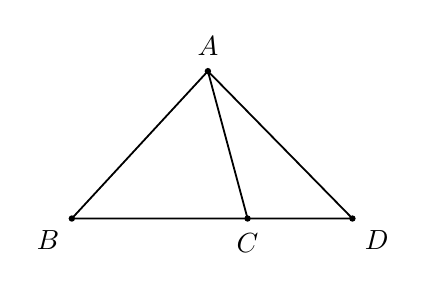
\begin{tikzpicture}[scale=.72,baseline=(current bounding box.center),line cap=round]
    \coordinate (A) at (0,2.6); \coordinate (B) at (-2.4,0);
    \coordinate (C) at (.7,0); \coordinate (D) at (2.55,0);
    \draw[black,line width=.65pt] (A)--(B)--(D)--cycle (A)--(C);
    \foreach \p in {A,B,C,D} \fill (\p) circle (1.6pt);
    \node[above=2pt] at (A) {$A$};
    \node[below left=1pt] at (B) {$B$};
    \node[below=2pt] at (C) {$C$};
    \node[below right=1pt] at (D) {$D$};
  \end{tikzpicture}
  \end{center}\vspace{-3mm}
  \fourchoices{$A,B,C$.}{$B,C,D$.}{$A,B,D$.}{$A,C,D$.}

\item \tdm{TDM21} Trên mặt phẳng hình vẽ cho năm điểm $A,B,C,D,E$ như hình vẽ.
  Đáp án \textbf{sai} là
  \begin{center}
  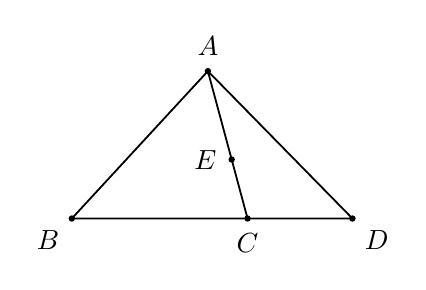
\begin{tikzpicture}[scale=.72,baseline=(current bounding box.center),line cap=round]
    \coordinate (A) at (0,2.6); \coordinate (B) at (-2.4,0);
    \coordinate (C) at (.7,0); \coordinate (D) at (2.55,0);
    \coordinate (E) at (.42,1.04);
    \draw[black,line width=.65pt] (A)--(B)--(D)--cycle (A)--(C);
    \foreach \p in {A,B,C,D,E} \fill (\p) circle (1.6pt);
    \node[above=2pt] at (A) {$A$};
    \node[below left=1pt] at (B) {$B$};
    \node[below=2pt] at (C) {$C$};
    \node[below right=1pt] at (D) {$D$};
    \node[left=2pt] at (E) {$E$};
  \end{tikzpicture}
  \end{center}\vspace{-3mm}
  \twochoices
  {$(AED)\equiv(BCD)$.}
  {$(ABC)\equiv(ABD)$.}
  {$(ABE)\equiv(ECD)$.}
  {$(EBD)\equiv(ACD)$.}

\item \tdm{TDM21} Mệnh đề nào dưới đây \textbf{sai}?
  \twochoices
  {Có một và chỉ một đường thẳng đi qua hai điểm phân biệt.}
  {Ba điểm không thẳng hàng xác định một mặt phẳng.}
  {Luôn tồn tại mặt phẳng đi qua bốn điểm bất kì trong không gian.}
  {Nếu đường thẳng $d$ có hai điểm nằm trên mặt phẳng $(\alpha)$ thì mọi điểm của $d$ đều nằm trên $(\alpha)$.}

\item \tdm{TDM21} Mệnh đề \textbf{sai} là
  \twochoices
  {Ba điểm không thẳng hàng xác định một mặt phẳng.}
  {Một đường thẳng và một điểm không thuộc nó xác định một mặt phẳng.}
  {Hai đường thẳng cắt nhau xác định một mặt phẳng.}
  {Bốn điểm trong không gian chắc chắn xác định ít nhất một mặt phẳng.}

\item \tdm{TDM21} Cho hình chóp $S.ABC$. Nhận xét \textbf{sai} là
  \twochoices
  {$SA,SB,SC$ là ba cạnh bên của hình chóp.}
  {Đỉnh của hình chóp là $S$.}
  {Ba tam giác $SAB,SBC,SCA$ là các mặt bên của hình chóp.}
  {$AB$ là một cạnh bên của hình chóp.}

\item \tdm{TDM21} Hãy chọn đáp án nhận xét \textbf{sai}. Một hình chóp tứ giác có
  \twochoices
  {Tất cả 4 mặt bên.}
  {Tất cả 5 đỉnh.}
  {Tất cả 4 cạnh bên.}
  {Duy nhất một mặt đáy.}

\item \tdm{TDM21} Cho hình chóp $S.ABCD$. Khi đó
  \twochoices
  {$ABCD$ là một tứ giác lồi.}
  {$SABC$ là một tứ giác.}
  {$SACD$ là một tứ giác lồi.}
  {$SABD$ là một tứ giác.}

\item \tdm{TDM21} Cho hình chóp $S.ABCD$. Khi đó
  \twochoices
  {Các tam giác $SAB,SAC,SBC$ là các mặt bên.}
  {$SBD$ là một mặt của hình chóp $S.ABCD$.}
  {Bốn điểm $A,B,C,D$ đồng phẳng.}
  {Hình chóp có tất cả 4 mặt.}

\item \tdm{TDM21} Chọn mệnh đề \textbf{sai} khi nói về hình chóp ngũ giác $S.ABCDE$?
  \twochoices
  {$ABCD$ là một hình tứ diện.}
  {$S.ABC$ là một hình chóp tam giác.}
  {$S.BCDE$ là một hình chóp tứ giác.}
  {$A,B,C,D,E$ đồng phẳng.}

\item \tdm{TDM21} Hình tứ diện $ABCD$ có tất cả
  \fourchoices{1 đỉnh.}{2 đỉnh.}{3 đỉnh.}{4 đỉnh.}

\item \tdm{TDM21} Hình tứ diện $ABCD$ có tất cả
  \fourchoices{4 cạnh.}{8 cạnh.}{6 cạnh.}{5 cạnh.}

\item \tdm{TDM21} Hình tứ diện $MNPQ$ có tất cả
  \fourchoices{6 mặt.}{4 mặt.}{3 mặt.}{5 mặt.}

\item \tdm{TDM21} Cho hình chóp tam giác $S.ABC$.
  Giao tuyến của hai mặt phẳng $(SAB)$ và $(SAC)$ là đường thẳng
  \fourchoices{$SA$.}{$AB$.}{$SB$.}{$BC$.}

\item \tdm{TDM21} Cho hình chóp tứ giác $S.ABCD$ có giao điểm của $AC$ và $BD$ là $O$.
  Giao tuyến của hai mặt phẳng $(SAC)$ và $(SBD)$ là đường thẳng
  \fourchoices{$AO$.}{$SA$.}{$OC$.}{$SO$.}

\item \tdm{TDM21} Cho hình chóp tứ giác $S.ABCD$ có đáy không phải hình thang.
  Giao tuyến của hai mặt phẳng $(SAB)$ và $(SCD)$ là đường thẳng
  \twochoices
  {$SA$.}
  {$SO$ với $O$ là giao điểm của $AC$ và $BD$.}
  {$SI$ với $I$ là giao điểm của $AB$ và $CD$ kéo dài.}
  {$SE$ với $E$ là giao điểm của $AD$ và $BC$ kéo dài.}

\item \tdm{TDM31} Cho hình chóp tam giác $S.ABC$.
  Gọi $M$ là trung điểm của $SA$ và $N$ là điểm nằm trên cạnh $SB$.
  Giao tuyến của hai mặt phẳng $(SMN)$ và đáy $(ABC)$ là đường thẳng
  \fourchoices{$MN$.}{$SA$.}{$SB$.}{$AB$.}

\pagebreak[4]
\item \tdm{TDM42 -- A} Cho tứ diện $ABCD$.
  Gọi $M$ là trung điểm của cạnh $AB$, $N$ là điểm nằm trên cạnh $AC$ sao cho
  $NA=3NC$, $Q$ là điểm nằm trên cạnh $BD$ sao cho $QB=4QD$.
  Gọi $P=CD\cap(MNQ)$. Tỉ số $\dfrac{PC}{PD}$ bằng
  \fourchoices{$\dfrac43$.}{$3$.}{$\dfrac32$.}{$\dfrac53$.}
\end{questions}

\vspace{2mm}
\textbf{PHẦN B. TỰ LUẬN (3 câu).}
\begin{questions}[resume]

\item \tdm{TDM32 -- TL} Cho tứ diện $ABCD$ và các điểm $M,N,P$ lần lượt thuộc các cạnh
  $AB,AC,AD$. Giả sử $NP$ và $CD$ cắt nhau tại $Q$, $PM$ và $DB$ cắt nhau
  tại $R$, $MN$ và $BC$ cắt nhau tại $S$.
  Hãy chứng minh rằng $Q,R,S$ thẳng hàng.

\item \tdm{TDM32 -- TL} Cho hình chóp $S.ABCD$ có đáy $ABCD$ không phải là hình thang.
  Gọi $M,N$ lần lượt là trung điểm của các cạnh $SA,SB$, gọi $P$ là điểm nằm
  trong tam giác $SCD$.
  \begin{enumerate}[label=\arabic*.,leftmargin=7mm,itemsep=1pt,topsep=2pt,parsep=0pt]
  \item Hãy tìm giao điểm của đường thẳng $MN$ và mặt phẳng $(SCD)$.
  \item Hãy tìm giao điểm của đường thẳng $MP$ và mặt phẳng $(SBC)$.
  \end{enumerate}

\item \tdm{TDM32 -- TL} Cho hình chóp $S.ABCD$ có đáy $ABCD$ không phải là hình thang.
  Gọi $M$ là điểm nằm trong tam giác $SCD$.
  \begin{enumerate}[label=\arabic*.,leftmargin=7mm,itemsep=1pt,topsep=2pt,parsep=0pt]
  \item Hãy xác định giao tuyến của hai mặt phẳng $(SBM)$ và $(SAC)$.
  \item Hãy xác định giao điểm của đường thẳng $BM$ và mặt phẳng $(SAC)$.
  \end{enumerate}
\end{questions}

\vspace{3mm}
\begin{center}\textbf{---------- HẾT ----------}\end{center}
\end{document}